\chapter{Исследовательский раздел}
\label{cha:research}

В данном разделе приведено сравнение алгоритмов по времени работы.
Все параметры замерялись на устройстве со следующими техническими характеристиками:
\begin{itemize}
	\item операционная система macOS Monterey 12.6 \cite{monterey};
	\item оперативная память 16 Гб;
	\item процессор 2,3 ГГц 8‑ядерный Intel Core i9 9 поколения \cite{intel}.
\end{itemize}

Во время замеров ноутбук был подключен к сети питания и нагружен только приложениями, использующимися при замерах.

\section{Измерение времени работы реализаций алгоритмов}

Процессорное время замерялось при помощи функции time из заголовочного файла time.h~\cite{cplusplus}. Результаты сформированы в виде графиков при помощи библиотеки matplotlib~\cite{matplotlib}.  Каждый алгоритм был выполнен 30 раз, а затем время усреднялось.
Время было замерено на случайно сформированных массивах.

Результаты замеров представлены в таблице \ref{tbl:timings}.

На рисунках \ref{fig:timings} на осях X указано количество элементов во входном массиве. Время на осях Y указано в секундах.

\begin{table}[h]
	\begin{center}
		\begin{threeparttable}
			\captionsetup{justification=raggedright,singlelinecheck=off}
			\caption{\label{tbl:timings} Результаты замеров}
			\begin{tabular}{|c|c|c|}
				\hline
				Количество частиц вируса& Время отрисовки сцены (в миллисекундах) \\  \hline
				1 & 235.0 \\ \hline 
				10 & 255.0 \\ \hline 
				20 & 265.0 \\ \hline 
				40 & 295.0 \\ \hline 
				60 & 330.0 \\ \hline 
				100 & 390.0 \\ \hline 
				150 & 460.0 \\ \hline 
				200 & 550.0 \\ \hline 
				250 & 620.0 \\ \hline 
				300 & 680.0 \\ \hline 
				400 & 830.0 \\ \hline 
				500 & 1000.0 \\ \hline 
				600 & 1130.0 \\ \hline 
			\end{tabular}
		\end{threeparttable}
	\end{center}
	
\end{table}

\begin{figure}[ph!]
	\center{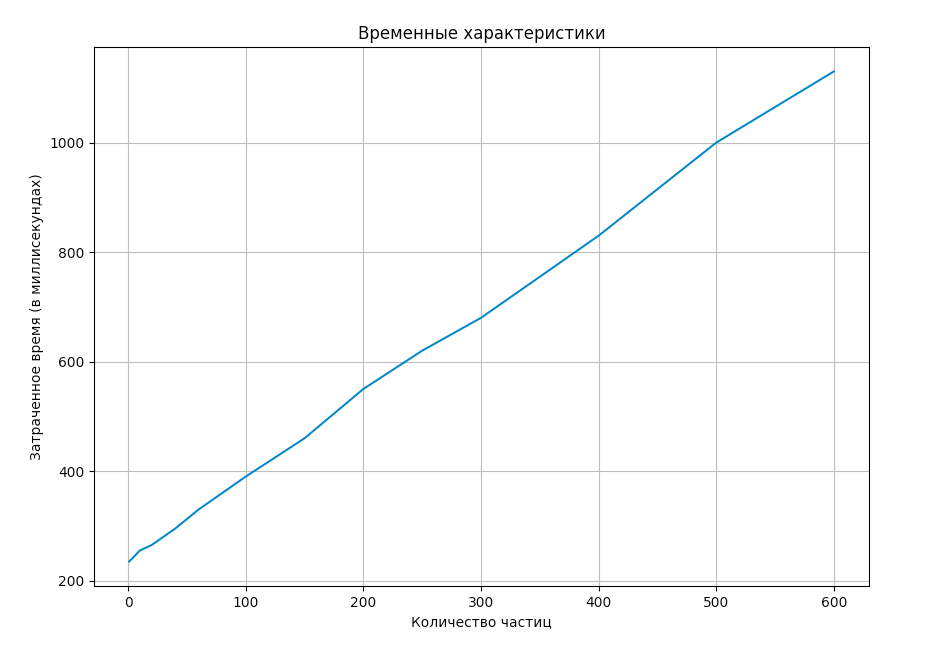
\includegraphics[scale=0.5]{img/timings.png}}
	\caption{Результаты замеров времени реализаций алгоритма битонной сортировки для разного количества потоков (количество элементов в массиве равно 1024)}
	\label{fig:timings}
\end{figure}

\clearpage

\section*{Вывод}

В результате эксперимента можно сделать вывод, что при использовании 8 потоков, многопоточная реализация алгоритма битонной сортировки лучше реализации без многопоточности в среднем на 35\% при количестве элементов в массиве равном 1024. 


